\section{Pão de Queijo}
\subsection*{Ingredients}
\begin{multicols}{2}
\begin{ingredients}
    \item 500g Tapioca Starch (250g \textit{Doce} / 250g \textit{Azedo})
    \item 250g Whole Milk (oat is fine)
    \item 100ml Water
    \item 100ml Vegetable Oil
    \item 10g Fine Salt
    \item 3 Eggs
    \item 150g Parmesan, finely grated
    \item 100g Mozzarella or mild cheddar, grated
\end{ingredients}
\end{multicols}

\subsection*{Recipe}
\begin{enumerate}
    \item Scald: Bring milk, water, oil, and salt to a rolling boil and pour over the starch. Stir until a lumpy, sticky paste forms.
    \item Cool: Allow the dough to cool for 15 minutes. It must be warm to the touch, not hot, to avoid scrambling the eggs.
    \item Mix: Incorporate eggs one at a time. Add the cheeses and knead until the dough is smooth, glossy, and uniform (\textit{massa lisa}).
    \item Form: Preheat oven to 190°C. Grease hands with oil and roll 30g balls. Space 5cm apart on a lined baking sheet.
    \item Bake: Bake for 20--25 minutes.
\end{enumerate}

\subsection*{Hints}
\begin{itemize}
    \item Texture Science: Scalding causes starch gelatinization ($T \approx 65^\circ C$), creating the elastic matrix that traps steam for the rise.
    \item Starch Ratio: 100\% \textit{Doce} (Sweet) yields a dense, chewy roll; 100\% \textit{Azedo} (Sour) creates a hollow, tangy, and very airy puff.
\end{itemize}

\vfill % Push to bottom
\begin{center}
    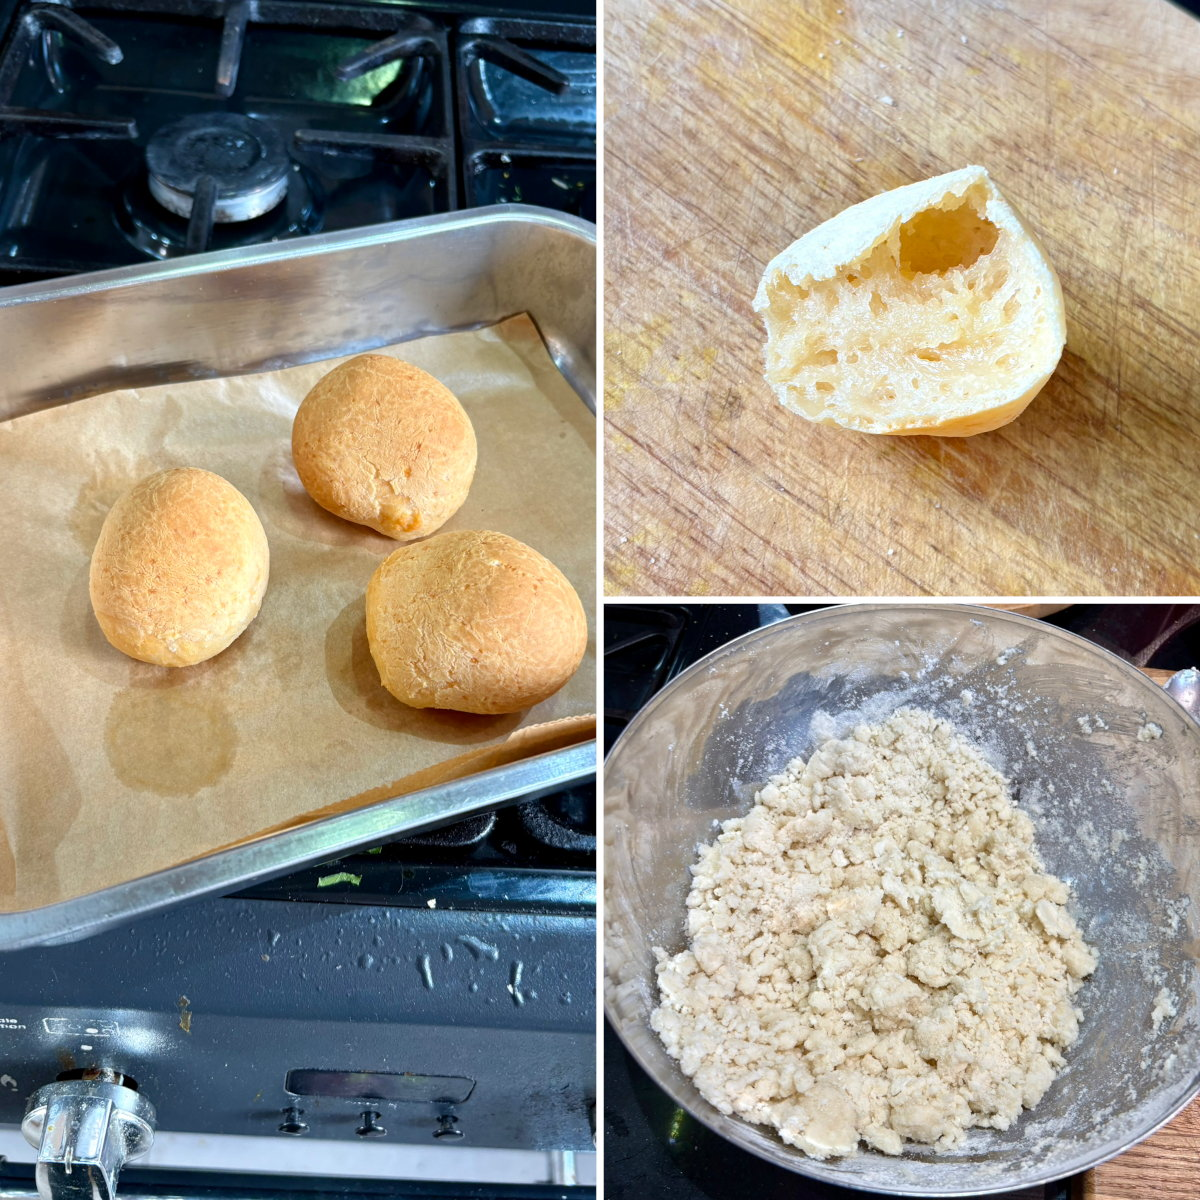
\includegraphics[
        width=\textwidth,
        height=\dimexpr\pagegoal-\pagetotal-2\baselineskip\relax,
        keepaspectratio
    ]{chapters/02_starters_and_sides/pao_de_queijo.jpg}
\end{center}
\newpage